\section{Tugas 1 -- Klasifikasi Cacat Multimodal}
Data latih: 48.000 unit dengan gambar permukaan $64\times64$ dan sinyal sensor penekanan $3\times128$ (suhu, getaran, arus); data uji 16.000 unit.
Metrik uji adalah macro-F1 tujuh kelas. Validasi memakai 20\% data latih yang dibagi bertingkat menurut kelas $\times$ lini.

\subsection*{(a) Eksplorasi}
Kelas sangat tidak seimbang: \emph{normal} \TsatuKelasNormal\% dan \emph{kontaminasi} hanya \TsatuKelasKontaminasi\% (Tabel~\ref{tab:t1_eda_kelas_missing}).
Gambar contoh tiap kelas dan rata-rata sinyal per kelas ada di Gambar~\ref{fig:t1gambar}--\ref{fig:t1sinyal}. Sensor tidak terekam utuh (ketiga kanal kosong) pada
\TsatuSensorHilang\% unit dan setidaknya satu kanal kosong pada \TsatuSensorSatuHilang\% unit; kekosongan selalu satu kanal penuh, tidak pernah sebagian.
\textbf{Perbedaan train--uji yang besar:} lini B hanya \TsatuLiniBTrain\% data latih tetapi \TsatuLiniBTest\% data uji, dan gambar lini B lebih gelap
(rata-rata piksel \TsatuPikselB{} vs \TsatuPikselA{} pada lini A; Gambar~\ref{fig:t1domain}). Mesin M01--M06 hanya ada di lini A dan M07--M12 di lini B.
Karena itu metrik utama validasi adalah \emph{F1 terbobot uji} $=0{,}4\,\mathrm{F1}_A + 0{,}6\,\mathrm{F1}_B$, yang meniru komposisi data uji.

\begin{figure}[ht]\centering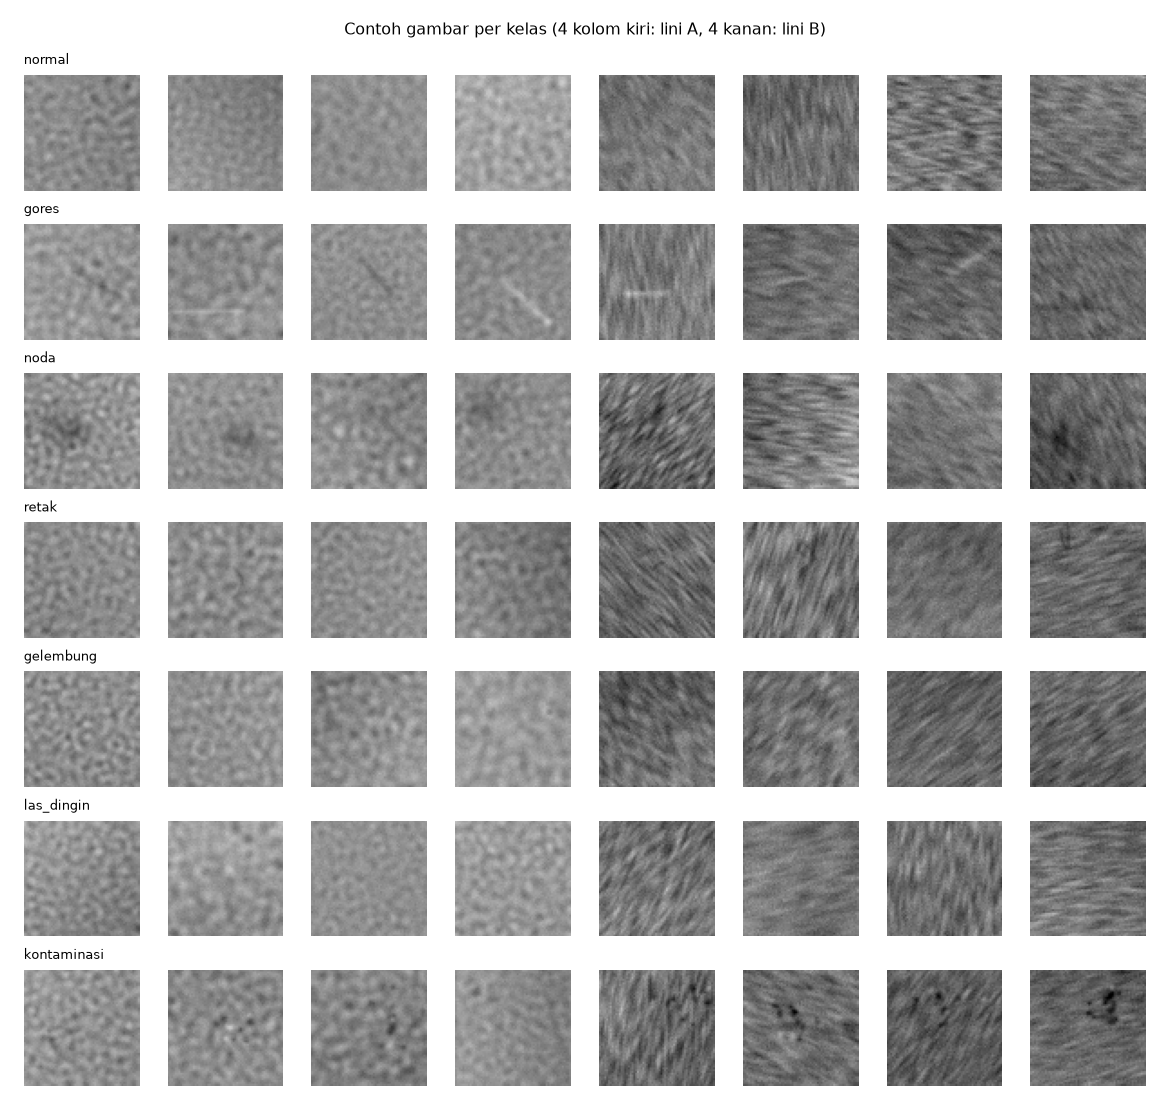
\includegraphics[width=.62\linewidth]{t1_eda_gambar.png}
\caption{Contoh gambar per kelas (kiri lini A, kanan lini B).}\label{fig:t1gambar}\end{figure}
\begin{figure}[ht]\centering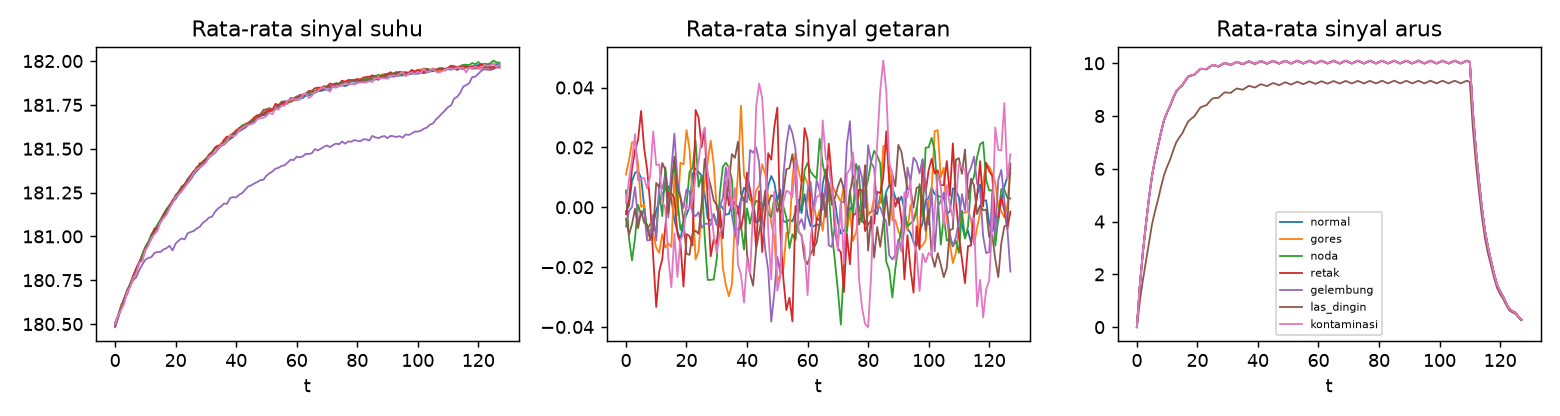
\includegraphics[width=\linewidth]{t1_eda_sinyal.png}
\caption{Rata-rata sinyal tiap kanal per kelas.}\label{fig:t1sinyal}\end{figure}
\begin{figure}[ht]\centering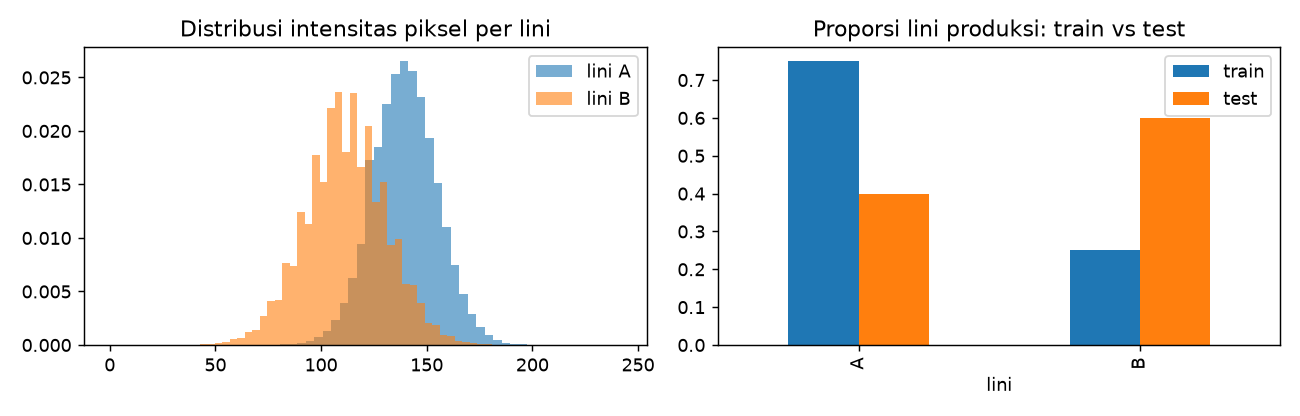
\includegraphics[width=.85\linewidth]{t1_eda_domain.png}
\caption{Intensitas piksel per lini dan proporsi lini di data latih vs uji.}\label{fig:t1domain}\end{figure}
\begin{table}[ht]
\centering\small
\resizebox{\ifdim\width>\linewidth\linewidth\else\width\fi}{!}{%
\begin{tabular}{lrrrrr}
\toprule
kelas & hilang\_suhu\_\% & hilang\_getaran\_\% & hilang\_arus\_\% & hilang\_semua\_\% & porsi\_kelas\_\% \\
\midrule
normal & 5.87 & 5.84 & 5.90 & 4.76 & 49.77 \\
gores & 6.30 & 6.31 & 6.24 & 5.18 & 11.71 \\
noda & 5.93 & 6.10 & 6.14 & 5.17 & 9.94 \\
retak & 6.43 & 6.52 & 6.63 & 5.55 & 7.51 \\
gelembung & 6.18 & 6.03 & 6.01 & 5.10 & 7.15 \\
las\_dingin & 5.78 & 5.69 & 5.57 & 4.70 & 9.01 \\
kontaminasi & 5.30 & 4.96 & 5.18 & 4.16 & 4.91 \\
\bottomrule
\end{tabular}
}
\caption{Distribusi kelas dan persentase kanal sensor yang tidak terekam per kelas.}
\label{tab:t1_eda_kelas_missing}
\end{table}


\subsection*{(b) Arsitektur dan strategi fusion}
\textbf{Encoder gambar:} CNN empat blok (konvolusi $3\times3$--BatchNorm--ReLU dua kali lalu max-pooling) yang menghasilkan peta fitur $256\times4\times4$;
rata-rata globalnya menjadi vektor 256 dimensi dan 16 posisinya menjadi token. \textbf{Encoder sinyal:} 1D-CNN tiga blok; masukannya tiga kanal sinyal
yang dinormalisasi ditambah tiga kanal \emph{mask} (1 = kanal tidak terekam) sehingga model tahu kanal mana yang hilang; keluarannya vektor 128 dimensi dan 16 token.
Tiga strategi fusion dibandingkan dengan seed dan anggaran epoch yang sama (Tabel~\ref{tab:t1_fusion}):
(i) \emph{concat} --- vektor kedua modalitas digabung lalu satu kepala klasifikasi (fusion tingkat fitur);
(ii) \emph{late fusion} --- kepala terpisah per modalitas, logit digabung dengan bobot per kelas yang dipelajari, dan bila seluruh sensor hilang keputusan otomatis dari gambar saja;
(iii) \emph{cross-attention} dua arah antara token gambar dan token sinyal.
Semua model dilatih dengan AdamW, jadwal one-cycle, bobot kelas $\sqrt{1/\text{frekuensi}}$, augmentasi flip/rotasi $90^\circ$, dan \emph{modality dropout}
(sensor dihapus seluruhnya dengan peluang 0,15 dan satu kanal dengan peluang 0,10). F1 terbobot uji: concat \TsatuFlConcat, late \TsatuFlLate, cross-attention \TsatuFlCross;
terpilih \textbf{\TsatuKonfigFusion}.

\begin{table}[ht]
\centering\small
\resizebox{\ifdim\width>\linewidth\linewidth\else\width\fi}{!}{%
\begin{tabular}{lrrrrr}
\toprule
model & f1\_macro & f1\_lini\_A & f1\_lini\_B & f1\_terbobot\_uji & epoch\_terbaik \\
\midrule
concat (early/feature-level) & 0.824 & 0.859 & 0.707 & 0.768 & 11 \\
late fusion & 0.855 & 0.887 & 0.750 & 0.805 & 10 \\
cross-attention & 0.855 & 0.894 & 0.733 & 0.797 & 11 \\
\bottomrule
\end{tabular}
}
\caption{Perbandingan strategi fusion (validasi). F1 terbobot uji = 0.4 F1 lini A + 0.6 F1 lini B.}
\label{tab:t1_fusion}
\end{table}


\subsection*{(c) Nilai tiap modalitas}
Model gambar saja mencapai F1 terbobot \TsatuFlImage{} dan sensor saja \TsatuFlSensor. Per kelas (Tabel~\ref{tab:t1_modalitas}, Gambar~\ref{fig:t1cm}):
kelas yang terutama dikenali dari \textbf{gambar}: \TsatuKelasGambar; dari \textbf{sensor}: \TsatuKelasSensor; yang baru terbaca baik setelah \textbf{fusion}: \TsatuKelasKeduanya.
Hal ini sesuai dengan sifat cacatnya: gores, noda, dan kontaminasi adalah cacat permukaan yang terlihat jelas di citra (Gambar~\ref{fig:t1gambar}), sehingga model sensor saja sama sekali tidak mengenalinya (F1 = 0). Sebaliknya, las dingin tidak tampak di permukaan (F1 gambar saja = 0) tetapi memiliki pola arus dan suhu yang khas saat penekanan (Gambar~\ref{fig:t1sinyal}), sehingga sensor saja sudah mencapai F1 0.93. Retak dan gelembung terbaca dari kedua modalitas, dan fusion menaikkan F1-nya di atas masing-masing modalitas.
\begin{table}[ht]
\centering\small
\resizebox{\ifdim\width>\linewidth\linewidth\else\width\fi}{!}{%
\begin{tabular}{lrrrl}
\toprule
kelas & image-only & sensor-only & fusion (late fusion) & modalitas\_utama \\
\midrule
normal & 0.841 & 0.737 & 0.906 & keduanya (fusion) \\
gores & 0.723 & 0.000 & 0.788 & gambar \\
noda & 0.875 & 0.000 & 0.882 & gambar \\
retak & 0.538 & 0.706 & 0.755 & sensor \\
gelembung & 0.648 & 0.772 & 0.799 & sensor \\
las\_dingin & 0.000 & 0.930 & 0.930 & sensor \\
kontaminasi & 0.913 & 0.000 & 0.924 & gambar \\
\bottomrule
\end{tabular}
}
\caption{F1 per kelas: image-only, sensor-only, dan fusion terpilih (validasi).}
\label{tab:t1_modalitas}
\end{table}

\begin{figure}[ht]\centering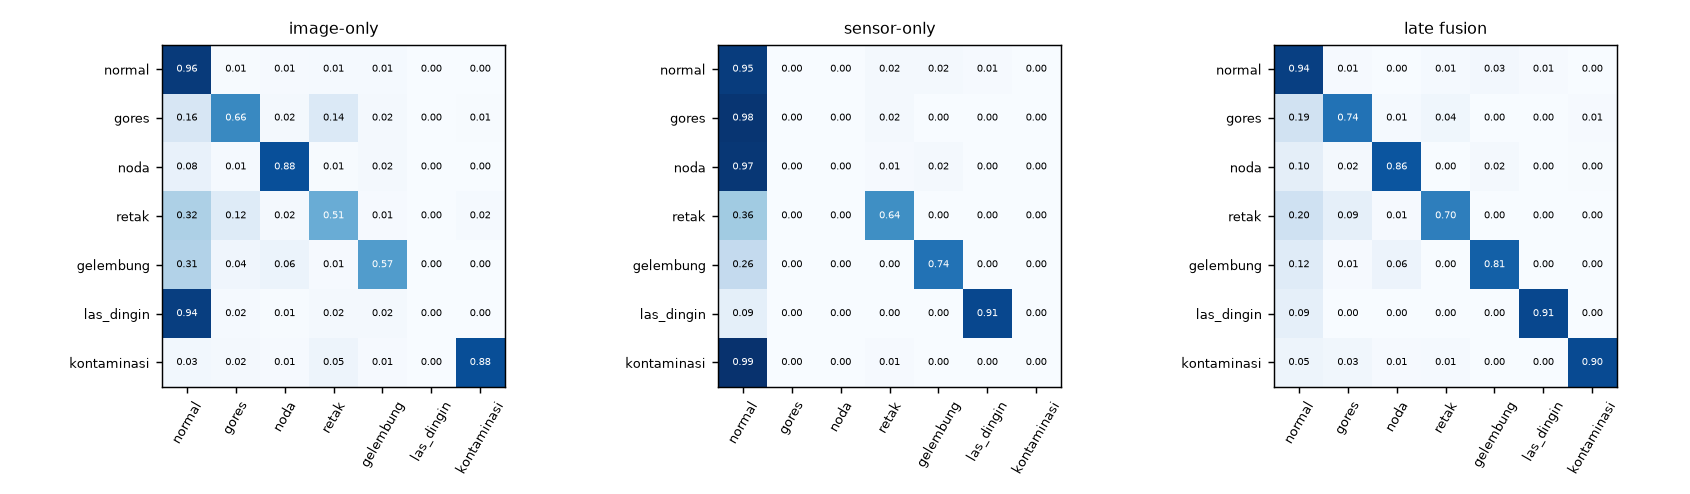
\includegraphics[width=\linewidth]{t1_confusion_modalitas.png}
\caption{Confusion matrix (dinormalisasi per kelas aktual) model gambar saja, sensor saja, dan fusion.}\label{fig:t1cm}\end{figure}

\subsection*{(d) Label tidak sempurna}
Kemungkinan salah label dideteksi dengan \emph{confident learning}: probabilitas \emph{out-of-fold} (3-fold) dari model fusion; ambang per kelas $t_j$ = rata-rata $p_j$ pada
sampel berlabel $j$; sampel dicurigai bila $p(\text{label}) < t_{\text{label}}$ sementara ada kelas lain $j$ dengan $p_j \ge t_j$.
Hasilnya \TsatuNoiseN{} sampel latih (\TsatuNoisePersen\%) dicurigai (Tabel~\ref{tab:t1_label_noise}, contoh di Gambar~\ref{fig:t1noise}).
Dua teknik robust diuji: \emph{label smoothing} 0,1 dan membuang sampel yang dicurigai (Tabel~\ref{tab:t1_robust_noise}). Karena label validasi sendiri bisa salah,
F1 juga dihitung pada validasi tanpa sampel yang dicurigai (\TsatuValBersihPersen\% validasi). Terpilih: \textbf{\TsatuKonfigNoise}.
Sampel yang dicurigai tidak tersebar merata. Menurut kelas, porsi tertinggi ada pada retak (25.4\%), kontaminasi (18.6\%), dan gores (13.8\%), dengan kelas kandidat tersering \emph{gores}; ini wajar karena ketiganya berupa pola garis atau bercak yang mirip secara visual. Menurut lini, porsinya lebih tinggi di lini A (8.8\%) dibanding lini B (5.2\%), dan terkonsentrasi pada mesin M01--M06 (7.9--9.4\%) dibanding M07--M12 (4.5--5.9\%). Sebaliknya, per shift hampir sama (7.7--8.1\%), sehingga kesalahan label kemungkinan berkaitan dengan proses inspeksi di lini/mesin tertentu, bukan dengan shift kerja.
\begin{table}[ht]
\centering\small
\resizebox{\ifdim\width>\linewidth\linewidth\else\width\fi}{!}{%
\begin{tabular}{lrrrl}
\toprule
kelas\_label & n & dicurigai & persen\_dicurigai & kelas\_kandidat\_tersering \\
\midrule
normal & 19110 & 672 & 3.52 & gores \\
gores & 4499 & 622 & 13.83 & normal \\
noda & 3818 & 280 & 7.33 & gores \\
retak & 2885 & 733 & 25.41 & gores \\
gelembung & 2744 & 267 & 9.73 & noda \\
las\_dingin & 3458 & 101 & 2.92 & normal \\
kontaminasi & 1886 & 351 & 18.61 & gores \\
\bottomrule
\end{tabular}
}
\caption{Sampel latih yang dicurigai salah label (confident learning, 3-fold out-of-fold).}
\label{tab:t1_label_noise}
\end{table}

\begin{figure}[ht]\centering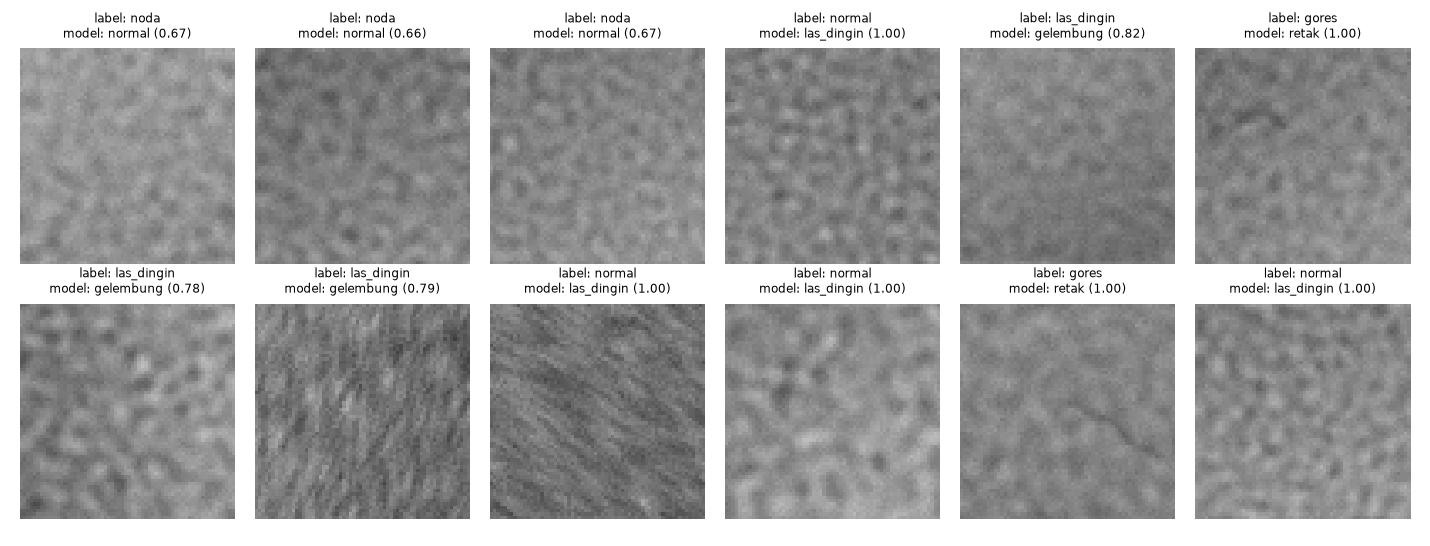
\includegraphics[width=.85\linewidth]{t1_label_noise_contoh.png}
\caption{Contoh sampel yang paling dicurigai salah label: label inspektur vs prediksi model.}\label{fig:t1noise}\end{figure}
\begin{table}[ht]
\centering\small
\resizebox{\ifdim\width>\linewidth\linewidth\else\width\fi}{!}{%
\begin{tabular}{lrrr}
\toprule
teknik & f1\_macro & f1\_terbobot\_uji & f1\_terbobot\_val\_bersih \\
\midrule
baseline (CE + bobot kelas) & 0.855 & 0.805 & 0.884 \\
label smoothing 0.1 & 0.855 & 0.806 & 0.879 \\
buang sampel dicurigai & 0.838 & 0.787 & 0.856 \\
\bottomrule
\end{tabular}
}
\caption{Teknik robust terhadap label noise (validasi penuh dan validasi tanpa sampel yang dicurigai).}
\label{tab:t1_robust_noise}
\end{table}


\subsection*{(e) Domain shift antar lini}
Tanpa penanganan, F1 lini A \TsatuDomFlA{} dan lini B \TsatuDomFlB{} (Tabel~\ref{tab:t1_domain}). Tiga teknik diuji: normalisasi intensitas per lini
(sah karena lini tercantum di metadata uji), augmentasi kecerahan/kontras acak, dan bobot sampel lini B $\times2$. Terpilih \textbf{\TsatuKonfigDomain}
(F1 lini B \TsatuDomBestFlB).

\begin{table}[ht]
\centering\small
\resizebox{\ifdim\width>\linewidth\linewidth\else\width\fi}{!}{%
\begin{tabular}{lrrrr}
\toprule
teknik & f1\_macro & f1\_lini\_A & f1\_lini\_B & f1\_terbobot\_uji \\
\midrule
tanpa penanganan & 0.855 & 0.887 & 0.753 & 0.806 \\
normalisasi per lini & 0.857 & 0.887 & 0.765 & 0.814 \\
augmentasi kecerahan/kontras & 0.853 & 0.887 & 0.745 & 0.802 \\
bobot sampel lini B $\times$2 & 0.848 & 0.876 & 0.758 & 0.806 \\
\bottomrule
\end{tabular}
}
\caption{Domain shift: F1 per lini dan F1 terbobot porsi uji untuk tiap teknik.}
\label{tab:t1_domain}
\end{table}


\subsection*{(f) Sensor yang tidak terekam}
Model final diuji dengan sensor asli, seluruh sensor dihapus, dan satu kanal acak dihapus (Tabel~\ref{tab:t1_missing}): F1 terbobot \TsatuMissAsli, \TsatuMissHilang, dan \TsatuMissSatu.
Berkat kanal mask dan modality dropout, prediksi tetap masuk akal saat sensor hilang; bandingkan dengan model gambar saja (\TsatuFlImage).

\begin{table}[ht]
\centering\small
\resizebox{\ifdim\width>\linewidth\linewidth\else\width\fi}{!}{%
\begin{tabular}{lrrrr}
\toprule
kondisi sensor & f1\_macro & f1\_lini\_A & f1\_lini\_B & f1\_terbobot\_uji \\
\midrule
asli & 0.857 & 0.887 & 0.765 & 0.814 \\
hilang & 0.618 & 0.659 & 0.485 & 0.555 \\
satu\_kanal\_hilang & 0.787 & 0.823 & 0.680 & 0.737 \\
aslinya tidak terekam (n=480) & 0.608 & 0.638 & 0.528 & 0.572 \\
\bottomrule
\end{tabular}
}
\caption{Model final (seed pertama) saat sensor lengkap, seluruhnya hilang, atau satu kanal hilang (validasi).}
\label{tab:t1_missing}
\end{table}


\subsection*{(g) Training: sanity check, learning curve, tiga seed}
Model fusion mampu menghafal satu batch berisi 64 sampel (loss akhir \TsatuOverfitLoss, akurasi \TsatuOverfitAkurasi\%; Gambar~\ref{fig:t1overfit}), tanda bahwa pipeline
data--model--loss benar. Learning curve (Gambar~\ref{fig:t1lc}) dipakai untuk memilih epoch terbaik (early stopping pada F1 terbobot uji).
Tiga seed menghasilkan macro-F1 \TsatuSeedMean{} $\pm$ \TsatuSeedStd{} dan F1 terbobot \TsatuSeedWMean{} $\pm$ \TsatuSeedWStd{} (Tabel~\ref{tab:t1_seed});
ensemble ketiganya (rata-rata softmax) mencapai \TsatuEnsFl{} (terbobot \TsatuEnsFlW) dan dipakai untuk prediksi uji.

\begin{figure}[ht]\centering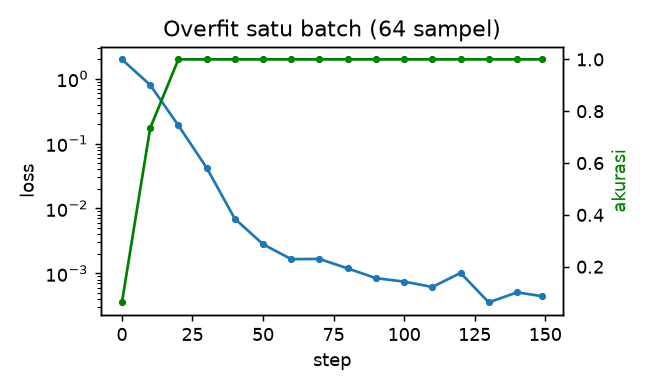
\includegraphics[width=.4\linewidth]{t1_overfit_batch.png}\hspace{1em}
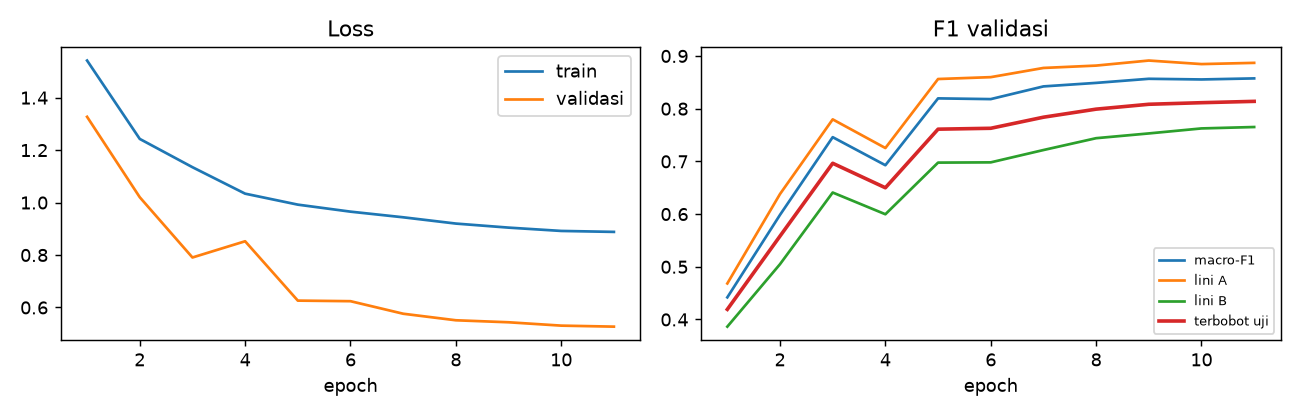
\includegraphics[width=.55\linewidth]{t1_learning_curve.png}
\caption{Kiri: overfit satu batch. Kanan: learning curve model final (seed pertama).}\label{fig:t1overfit}\label{fig:t1lc}\end{figure}
\begin{table}[ht]
\centering\small
\resizebox{\ifdim\width>\linewidth\linewidth\else\width\fi}{!}{%
\begin{tabular}{rrrrrr}
\toprule
seed & f1\_macro & f1\_lini\_A & f1\_lini\_B & f1\_terbobot\_uji & epoch\_terbaik \\
\midrule
42 & 0.857 & 0.887 & 0.765 & 0.814 & 11 \\
43 & 0.860 & 0.894 & 0.756 & 0.811 & 11 \\
44 & 0.857 & 0.890 & 0.753 & 0.808 & 11 \\
\bottomrule
\end{tabular}
}
\caption{Model final dengan 3 seed (validasi).}
\label{tab:t1_seed}
\end{table}

